%!TEX root = aust_thesis.tex
%%%%%%%%%%%%%%%%%%%%%%%%%%%%%%%%%%%%%%%%%%%%%%%%%%%%%%%%%%%%%%%%%%%%%%%
\chapter{Results and analysis}\label{ch:Results}


\section{Used Technologies}
Various technologies, frameworks and libraries were used in this project. Every implementation was carried out in Python, and frameworks like TensorFlow and Keras were used. Below are the list of the technologies used and a brief description.

\subsection{Python}

\begin{figure}
    \centering
    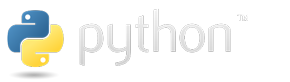
\includegraphics[width=0.7\linewidth]{images/python-logo.png}
     \caption{Python logo, source: https://www.python.org/community/logos/}
  \end{figure}

Python\footnote{https://www.python.org/community/logos/} is a high level programming language designed by Guido van Rossum in 1991. Its design philosophy emphasizes code readability and has a remarkable use of significant whitespace. The filename extensions include .py, .pyc, .pyw, .pyz. It support web development with frameworks like Django and Pyramid. It is applied in scientific studies and machine learning. Several libraries and frameworks have been developed by the Python community for this such as 
SciPy\footnote{www.scipy.org}, Scikit-learn\footnote{scikit-learn.org/stable/}, Pandas\footnote{pandas.pydata.org}, Numpy\footnote{www.numpy.org/}, Theano\footnote{deeplearning.net/software/theano/}, PyTorch \footnote{pytorch.org/}, etc. It is also one of the most popular languages in the field of Convolutional neural network. Neural Networks like ResNet, VGGNet, Faster R-CNN, AlexNet in Keras or Pytorch, etc. 

\subsection{ TensorFlow}
\begin{figure}
    \centering
    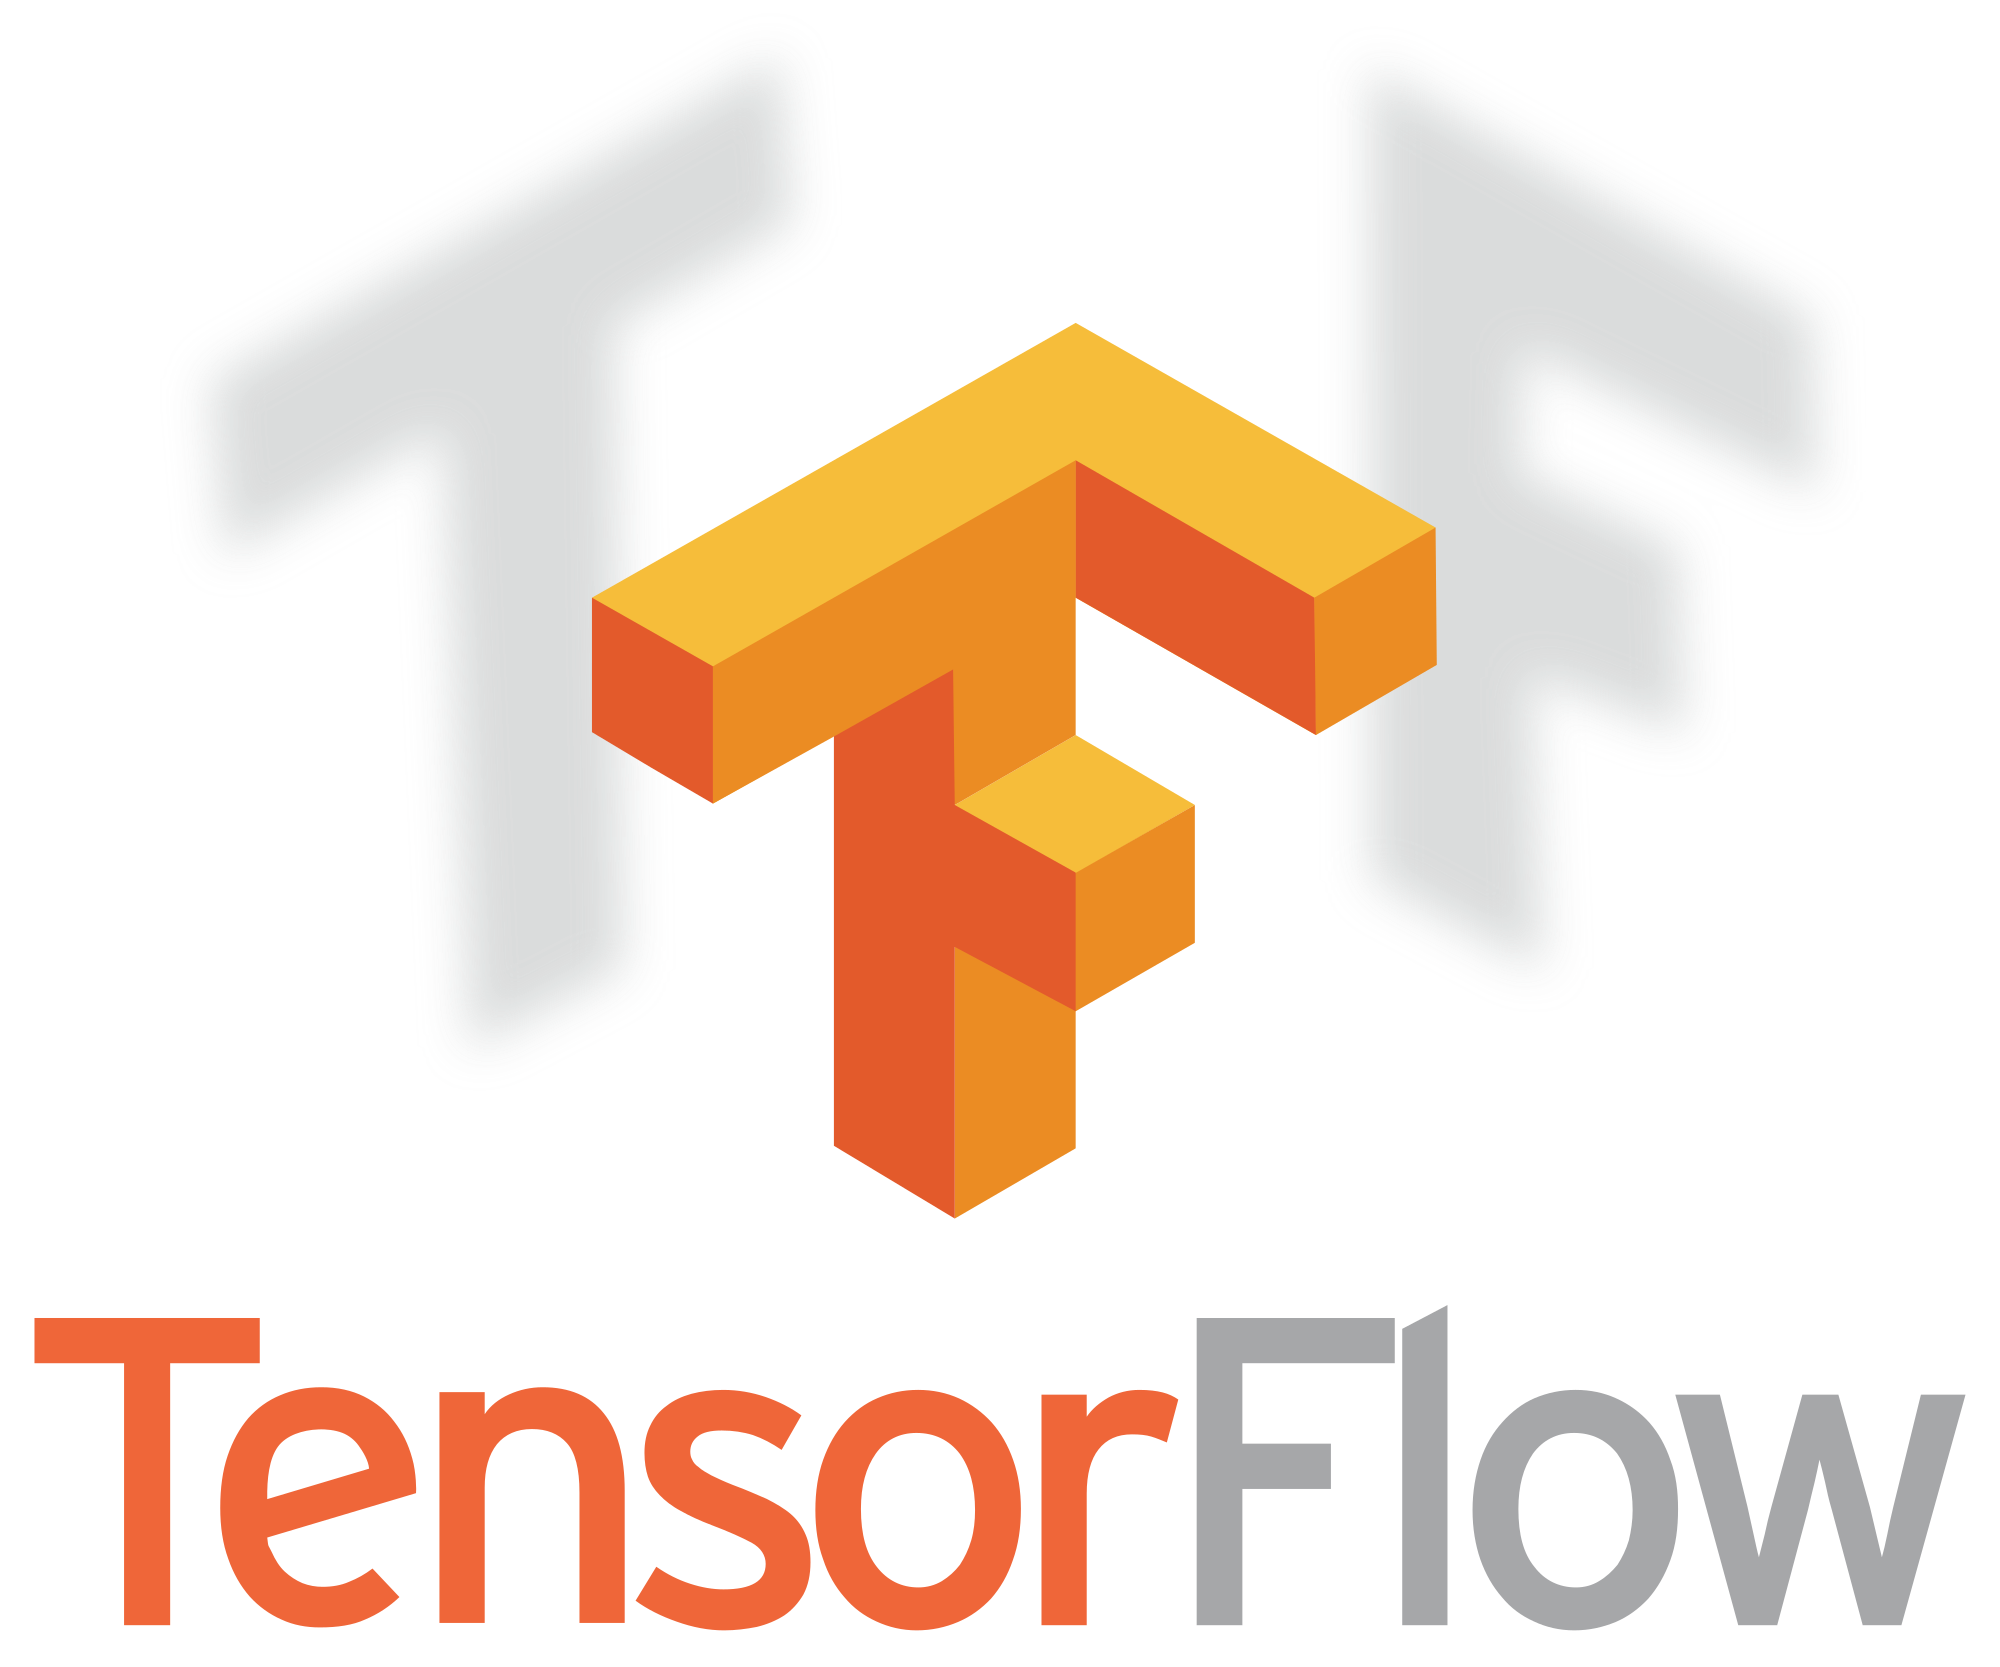
\includegraphics[width=0.7\linewidth]{images/TensorFlow.png}
     \caption{TensorFlow logo, source: www.tensorflow.org}
  \end{figure}
TensorFlow\footnote{www.tensorflow.org} is an Apache Licensed library. It is free and open-sourced and developed by Google Brain Team. It is written in Python, C++ and CUDA. It is a symbolic math library applied for machine learning application such as deep neural network, convolutional neural network. TensorFlow was used in the implementation of the deep learning network for this project. TensorFlow has a comprehensive, flexible ecosystem of tools, libraries that makes it user-friendly.

\subsection{Keras}
\begin{figure}
    \centering
    
\includegraphics[width=0.7\linewidth]{images/keras.png}
     \caption{Keras logo, source: www.keras.io}
  \end{figure}

Keras \footnote{Keras.io} is an MIT licensed neural-network library written in Python. It was design by Francois Chollet and released first in March 2015. It is open-sourced. Keras is capable of running on top of Microsoft Cognitive Toolkit, TensorFlow, PlaidML or Theano for fast experimentation of deep neural networks. It enables implementation of deep learning and allows easy and 
fast prototyping, supports both convolutional networks and recurrent networks and the combination of both.